\documentclass[a4paper]{article}
\author{Simon Wehrli}
\date{28.4.2013}
\title{Set similarity with b-bit k-permutation Minwise Hashing - DRAFT}

\usepackage[parfill]{parskip}
\usepackage{tikz} % for drawing advanced matrices
\usepackage{amsmath}
\usepackage{amsthm}
\usepackage{algorithm}
\usepackage{algorithmicx}
\usepackage{algpseudocode}
\usepackage{natbib}
\usepackage{tabulary}
\usepackage{caption}
\usepackage{framed}
\usepackage[english]{varioref} %automatische Anpassung von Referenzen
\labelformat{equation}{equation~(#1)} %make references to equations like (1)
\usepackage{float} % bewirkt, dass Option [H] für float-Umgebungen von Latex umgesetzt wird

\usetikzlibrary{matrix,decorations.pathreplacing,backgrounds,positioning}

\DeclareMathOperator{\Var}{Var}
\DeclareMathOperator{\E}{E}

\renewcommand{\algorithmicrequire}{\textbf{Input:}}
\renewcommand{\algorithmicensure}{\textbf{Output:}}

\newtheorem{mydef}{Definition}
\newtheorem{mylemma}{Lemma}
\newtheorem{mytheorem}{Theorem}

\begin{document} 
\maketitle

\section{Introduction}
This report is written for the seminar titled ``Algorithms for Database Systems" at ETH Z\"{u}rich. The seminar participants read and summarize various papers, which treat solving problems in the context of Big Data, which is this year's topic. This report summarizes and explains the core concepts of \citep{LiK11} and \citep{LiOwZhang12}.

With Big Data, most problems emphasis shifts from computational complexity to memory space usage considerations. Typically, the runtime is dominated by the time needed for memory accesses, hence optimizing the memory footprint already improves our algorithms significantly. 

Many today's applications are faced with very large datasets. A common task is to find \emph{similarity} between two or several such sets. There are lots of problem solutions which use a mapping to sets of properties and then do a \emph{similarity search} on them. Fast (approximative) algorithms for this search enable improvements of many well-known algorithms, e.g. of machine learning and computer vision.

We start by explaining the original \emph{Minwise Hashing}, which nicely presents the basic idea behind all algorithms. We move on to a major improvement, the \emph{b-bit k-permutation Minwise Hashing}, which reduces storage at the cost of more iterations in the algorithm and is a generalization of the concept. We then present \emph{One Permutation Hashing}, which manages surprising accuracy with just one run.

\subsection{Similarity}
We denote by $\Omega$ the set of all possible items of the sets $S_i \subseteq \Omega$, $i = 1 \text{ to } n$. $\left| \Omega \right| = D$ is always large (e.g. $D=2^{64}$). Often we consider only two sets $S_1 = X$, $S_2 = Y$.
\begin{framed}
\begin{mydef}\label{def:jaccard}
The normalized similarity between two sets $X$ and $Y$, known as \emph{resemblance} or \emph{Jaccard similarity}, denoted by R, is
\begin{equation}
R=\frac{\left| X \cap Y \right|}{\left| X \cup Y \right|} = \frac{a}{\left| X \right| + \left| Y \right| -a}, \qquad \text{where } a=\left| X \cap Y \right|
\end{equation}
\end{mydef}
\end{framed}

\subsection{Motivating Example}
Consider a web search provider, which want to present a result list of web pages without duplicates. To achieve that, for every pair of web pages, we drop one of them, if they are textually very similar. This is the case when their \emph{resemblance} $R$ is greater than some threshold $R_0$. But to be able to use the \emph{resemblance} as a measurement, we have to map each page to a set. One could imagine to define this mapping from the page to the set of all words occurring on the page. As in several studies \citep{Broder:1998,BroderGMZ97} we will instead map a page to a set of \emph{shingles}. A shingle is a string of $w$ contiguous words, and we include a \emph{shingle} in our result set if the \emph{shingle} occurs on the page (in the same order). Typically we choose $w = 5$. Figure \vref{fig:shingle} shows an exemplary mapping.

\begin{figure}[h]
\begin{center}
\fbox{
\parbox{2cm}{
This web page is just an example.
}
}
\hspace{1cm} $\underrightarrow{\text{mapping}}$ \hspace{1cm}
\parbox{2cm}{
\begin{equation*}
\begin{split}
 \text{\{} & \text{"This web page"},\\ & \text{"web page is"},\\ & \text{"page is just"},\\ & \text{"is just an"},\\ & \text{"just an example"} \text{\}}
\end{split}
\end{equation*}
}
\end{center}
\caption{The mapping from a web page to a set of \emph{shingles}.}
\label{fig:shingle}
\end{figure}

Clearly, the number of possible shingles and therefore $D$ is huge. Assume $10^5$ different English words, we have $D=\left(10^5\right)^5 \in \Theta\left(2^{25}\right)$. Thus computing the exact similarities for all pairs of pages of a web search would require prohibitive storage. For a single pair, we would already need $\Theta(D)$ storage.

\subsection{Original Minwise Hashing}

A working approximative solution to this problem was described by Broder and his colleagues \citep{Broder:1998,BroderGMZ97}. Their algorithm is based on the following observation:

Suppose a random permutation $\pi$ is performed on $\Omega$,
\[
\pi:\Omega \longrightarrow\ \Omega, \qquad \text{where } \Omega = \{0,1,\ldots,D-1\}.\footnote{We assume there is a perfect hash function applied to the elements of the original domain which always gives us $\Omega = \{0,1,\ldots,D-1\}$. Note that in the paper \citep{LiK11}, the hash function is applied after the permutation and the minimum-function, but it is simpler to understand this way.}
\]

With $\pi(S_i)$ we denote the application of the permutation $\pi$ to every element of $S_i$. A key role play the minima of the permuted sets:
\[
e_{S_i,\pi}=min(\pi(S_i))
\]

We use $\Pr[\cdot]$ as a shorthand for the \emph{Probability} of some event. An elementary probability argument shows that for two sets $X,Y \subseteq \Omega$
\begin{equation}\label{eq:minwiseOri}
\Pr[e_{X,\pi}=e_{Y,\pi}]=\Pr [\min(\pi(X))=\min(\pi(Y))]=\frac{\left| X \cap Y \right|}{\left| X \cup Y \right|}=R.
\end{equation}

We can now build an unbiased estimator $\hat{R}_M$ of $R$ with $k$ minwise independent permutations, $\pi_1,\pi_2,\ldots,\pi_k$:
\begin{equation}
\hat{R}_M=\frac{1}{k}\sum_{j=1}^k 1 \left\lbrace e_{X,\pi_j}=e_{Y,\pi_j} \right\rbrace,
\end{equation}
\begin{equation}\label{eq:minWiseVariance}
Var(\hat{R}_M)=\frac{1}{k}R(1-R).
\end{equation}
We later refer to $e_{S_i,\pi_j}$ as a \textbf{sample} and to $k$ as the \textbf{sample size}. To store a \textbf{sample} may require e.g., $64$ bits. Note that the minimum function $\min(\cdot)$ needs $O(D)$ time and constant space and can be precomputed for each set $S_i$ and permutation $\pi_j$.\footnote{A detailed runtime analysis will follow for the improved algorithm in section \vref{sec:b-bitMinwiseHashing}}

Many applications, especially duplicate detection, are interested in detecting somewhat high similarity, thus an approximation seems reasonable. From equation \vref{eq:minWiseVariance} we learn, that the accuracy can be adjusted by choosing the \textbf{sample size} appropriately.

However, finding duplicates out of $m$ objects, e.g. web pages, still needs $O(m^2)$ comparisons. There are number of approaches to deal with that problem, but we will not discuss it here and refer to \citep{BroderGMZ97,STOC02*380}.


\section{b-bit k-permutation Minwise Hashing}\label{sec:b-bitMinwiseHashing}

We will present an algorithm which improves on the storage requirements of the original \emph{Minwise Hashing}. The idea is to reduce the size of each \textbf{sample} by only taking $b$ bits of it, as opposed to, e.g. $64$ bits. Intuitively, this will increase the estimation variance $Var(\hat{R}_M)$, at the same \textbf{sample size} $k$. To maintain the same accuracy, we have to increase $k$. One can show, if the resemblance is not too small, we will not have to increase $k$ much and in total use less storage.

For example, when $b=1$ and $R=0.5$, the estimation variance will increase at most by a factor of $3$. To keep the same accuracy, we have to increase the \textbf{sample size} by a factor of $3$. If we before stored each minimum $\min(\pi_j(S_i))$ using $64$ bits, the improvement with $b=1$ is $64/3=21.3$.

Consider again two sets $X,Y \subseteq \Omega$, on which a random permutation $\pi: \Omega \longrightarrow \Omega$ is applied. We extend our notation with
\[
e_{X,b,\pi}=b \text{ lowest bits of } \min(\pi(X))
\]
\[
e_{Y,b,\pi}=b \text{ lowest bits of } \min(\pi(Y))
\]
\begin{framed}
\begin{mytheorem} \label{the:b-bitMinwiseHashing}
Assume $D$ is large.
\begin{equation}\label{eq:minwiseB-bit}
P_b=\Pr[1\left\lbrace e_{X,b,\pi}=e_{Y,b,\pi}\right\rbrace]=C_{1,b}+(1-C_{2,b})R
\end{equation}
\begin{equation}
r_X=\frac{|X|}{D}, \qquad r_Y=\frac{|Y|}{D}
\end{equation}
\begin{equation}
\begin{split}
C_{1,b}=A_{X,b}\frac{r_Y}{r_X+r_Y}+A_{Y,b}\frac{r_X}{r_X+r_Y},\\
C_{2,b}=A_{X,b}\frac{r_X}{r_X+r_Y}+A_{Y,b}\frac{r_Y}{r_X+r_Y}
\end{split}
\end{equation}
\begin{equation}
A_{X,b}=\frac{r_X[1-r_X]^{2^b-1}}{1-[1-r_X]^{2^b}}, \qquad A_{Y,b}=\frac{r_Y[1-r_Y]^{2^b-1}}{1-[1-r_Y]^{2^b}}
\end{equation}
\end{mytheorem}
\end{framed}

The intuition for the additional terms $C_{1,b}$ and $C_{2,b}$ in \vref{eq:minwiseB-bit} compared to \vref{eq:minwiseOri} is that we have to account for a type of "false positive": When two minima agree on their last $b$ bits, $e_{X,b,\pi}=e_{Y,b,\pi}$, it's still possible that their are different, $e_{X,\pi}\neq e_{Y,\pi}$. Thus even when $R=0$, the collision probability $P_b$ is not zero, but rather $C_{1,b}$. This makes the derivation much more complicated. A proof of Theorem \vref{the:b-bitMinwiseHashing} can be found in the appendix of \citep{LiK09}.

Even though $D$ is assumed to be large, experiments show that even for $D=20$ the absolute error caused by using \vref{eq:minwiseB-bit} ist $< 0.01$.

\subsection{The Estimator}

From \vref{eq:minwiseB-bit} of Theorem \vref{the:b-bitMinwiseHashing} we derive the estimator $\hat{R}_b$ for $R$:
\begin{equation}
\hat{R}_b=\frac{\hat{P}_b-C_{1,b}}{1-C_{2,b}}
\end{equation}
\begin{equation}
\hat{P}_b = \frac{1}{k}\sum_{j=1}^k 1 \left\lbrace  e_{X,b,\pi_j } = e_{Y,b,\pi_j } \right\rbrace
\end{equation}

This estimator is unbiased, i.e. $\E[\hat{R}_b]=\E[R]$. Furthermore, the variance of $\hat{R}_M$ converges to the variance of $\hat{R}_b$, i.e.
\begin{equation}
\lim_{b\rightarrow\inf}\Var\left(\hat{R}_b\right)=\frac{R(1-R)}{k}=\Var\left(\hat{R}_M\right)
\end{equation}

\subsection{Algorithm}

Based on the theoretical results, Algorithm \vref{alg:minwiseHashing} presents the procedure of $b$-bit ($k$-permutation) hashing.

\begin{algorithm}[H]
\caption{\textsc{b-bit Minwise Hashing} algorithm, applied to estimating pairwise resemblances in a collection of $n$ sets.}
\label{alg:minwiseHashing}
\begin{algorithmic}
\Require Sets $S_i \subseteq \Omega = \{0,1,\ldots,D-1\}, i = 1 \text{ to } n$. \Comment $D = \left| \Omega \right|$
\Ensure Estimated resemblance $\hat{R}_b$
\State // Pre-processing
\State Generate $k$ random permutations $\pi_j: \Omega\longrightarrow\Omega, j=1\text{ to }k$
\ForAll{$i = 1 \text{ to } n, j = 1 \text{ to } k$}
	\State Store the lowest $b$ bits of $\min(\pi_j(S_i))$, denoted by $e_{S_i,b,\pi_j}$.
\EndFor
\State
\State // Estimation (Use two sets $X,Y$ as an example)
\State Compute $\hat{P}_b = \frac{1}{k}\sum_{j=1}^k 1 \left\lbrace  e_{X,b,\pi_j } = e_{Y,b,\pi_j } \right\rbrace$
\State Estimate the resemblance by $\hat{R}_b = \frac{\hat{P}_b-C_{1,b}}{1-C_{2,b}}$, where $C_{1,b}$ and $C_{2,b}$ are from Theorem \vref{the:b-bitMinwiseHashing}
\end{algorithmic}
\end{algorithm}


\subsection{Deriving the Hamming Distance} \label{sec:hammingDistance}

Another well-known measurement for the similarity is the \emph{hamming distance}. For the purpose of calculating the \emph{hamming distance} between two sets $X,Y \subseteq \Omega = \{0,1,\ldots,D-1\}$, the sets are first mapped to a $D$-dimensional binary vector $x,y$ resp.:
\begin{framed}
\begin{mydef}\label{def:hamming}
Let vector $x,y \in \left\lbrace 0,1 \right\rbrace ^D, \, x_t = 1\left\lbrace t \in X \right\rbrace, y_t = 1\left\lbrace t \in Y \right\rbrace$. The \emph{hamming distance} between $X$ and $Y$ is
\begin{equation}
H=\sum_{i=0}^{D-1}\left[ x_i \neq y_i \right]=|X \cup Y|-|X\cap Y|=|X|+|Y|-2a
\end{equation}
\end{mydef}
\end{framed}

If we reformulate \vref{def:jaccard} as
\begin{equation}
a=\frac{R}{1+R}(|X|+|Y|),
\end{equation}
we can use the b-bit minwise hashing algorithm to estimate $H$ with
\begin{equation}
\hat{H}_b=|X|+|Y|-2\frac{\hat{R}_b}{1+\hat{R}_b}(|X|+|Y|)=\frac{1-\hat{R}_b}{1+\hat{R}_b}(|X|+|Y|)
\end{equation}

Experiments show that this approach is significantly faster than standard methods for computing the \emph{hamming distance}.

\subsection{Drawbacks}

The major problem of \emph{b-bit Minwise Hashing} is the costly preprocessing. Consider an application in machine learning, where the sets $S_i$ represents some properties of an object (e.g. a document or an image). Often one wants to add objects dynamically at runtime and compare them to other objects by finding the \emph{resemblance} of their properties. Finding the $k$ minima under the permutations may take too long, i.e. uses $O(k|S_i|)$ to $O(kD)$ time per set.
In general, the costly preprocessing may cause problems in user-facing applications, where the testing efficiency for new data objects is crucial. There is the need for a entirely fast algorithm to keep this applications responsive.

Another drawback is that storing $k$ permutations is sometimes impractical. If e.g. $D=10^9$, one permutation vector uses $4$GB, which is still possible. But the space needed to store e.g. $k=500$ permutation vectors (each of length $D$), is not tolerable.

%\begin{center}
\begin{table}
{\scriptsize 
\begin{tabulary}{1\textwidth}{LLL}
%\begin{tabular}{|l|l|l|l|l|}
\hline \textbf{Algorithm}  %& \textbf{Type} & \textbf{Space complexity} 
& \textbf{Pros} & \textbf{Cons} \\ 
\hline Karp, Shenker %& Deterministic %& $O\left(\frac{1}{s}\right)$ 
& Low memory usage.\newline Constant amortized time complexity per element. & No guarantees regarding false positives.\newline Requires two passes to find I(x,s) exactly.\newline Does not handle deletes.\newline Singleton streams only. \\ 
\hline Manku, Motwani (StickySampling) %& Randomized 	%& $O\left(\frac{1}{\varepsilon}\log \left(\frac{1}{s \cdot \delta}\right)\right)$ 
& Strong guarantees. & Worse average space complexity than LossyCounting.\newline Does not handle deletes. \\ 
\hline Manku, Motwani (LossyCounting) %& Deterministic %& $O\left(\frac{1}{\varepsilon}\log (\varepsilon \cdot n)\right)$ 
& Strong guarantees.\newline Good average space complexity.\newline Can be extended to handle itemsets.  & Does not handle deletes. \\ 
\hline Cormode, Muthukrishnan  %& Randomized 	%& $O\left(\frac{1}{s} \log\left(\frac{1}{s\cdot \delta}\right) \log m\right)$ 
& Handles deletes.\newline Moderate guarantees. & Singleton streams only.\newline False negatives possible.\newline Requires bijection to integers. \\ 
\hline 
%\end{tabular} 

\end{tabulary}
}
\caption{Algorithm comparison}
\label{ComparisonTable}
\end{table}
%\end{center}




\section{One Permutation Hashing}

This algorithm is directly motivated by the optimization potential of the standard \emph{minwise hashing} practice: intuitively, it ought to be "wasteful" in that all elements in a set are permuted, scanned but only the minimum will be used. As the name already suggests, we reduce the preprocessing step to only one permutation.

As in section \vref{sec:hammingDistance} we will represent sets $S_i \subseteq \Omega$ as vectors $s_i \in \left\lbrace 0,1 \right\rbrace ^D, \, (s_i)_t = 1\left\lbrace t \in S_i \right\rbrace$. We will setup a running example with $X,Y,Z \subseteq \Omega = \left\lbrace 0,1,\cdots,15\right\rbrace$. Let
\[
X=\left\lbrace 2,4,7,13\right\rbrace, \quad Y=\left\lbrace 0,3,6,13\right\rbrace, Z=\quad \left\lbrace 0,1,10,12\right\rbrace.
\]
Now we build up a data matrix where the rows are equal to the vector representations of the permuted sets:

\begin{equation}
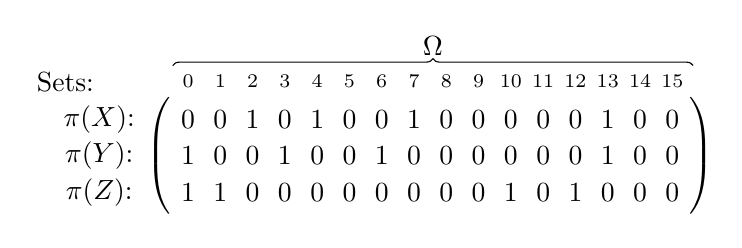
\begin{tikzpicture}[baseline = (M.center),% center with respect to the matrix center
        every left delimiter/.style={xshift=1ex},%tighter delimiter spacing
        every right delimiter/.style={xshift=-1ex}]
\matrix (M) [matrix of math nodes,left delimiter={(},right delimiter={)} 
        ]{ 
0&0&1&0&1&0&0&1&0&0&0&0&0&1&0&0\\
1&0&0&1&0&0&1&0&0&0&0&0&0&1&0&0\\
1&1&0&0&0&0&0&0&0&0&1&0&1&0&0&0\\
};
\node[anchor=south east] (cornernode) at (M-1-1.north west) {Sets: \qquad \qquad}; %Position this more precisely if desired
\foreach[count=\xi] \x in {0,1,2,3,4,5,6,7,8,9,10,11,12,13,14,15}{ %\xi is the counter \x is the value
\node[font=\scriptsize] (M-0-\xi) at (cornernode -| M-1-\xi) {\x}; % Gets the top row 
}

\foreach[count=\xi] \x in {$\pi(X)$:,$\pi(Y)$:,$\pi(Z)$:}{ %\xi is the counter \x is the value
\node (M-\xi-0) at (cornernode |- M-\xi-1) {\x}; %Gets the left most column
}

\draw[decoration=brace,decorate] (M-0-1.north west) -- (M-0-16.north east)%
 node[midway,above] {$\Omega$};

\end{tikzpicture}
\end{equation}

The idea is now to divide the columns evenly into $k$ (here $k=4$) bins (parts), and take the minimum in each bin. Because we only compare them within one bin, we can also re-index the elements to use the smallest possible representation of the minima:

\begin{equation}
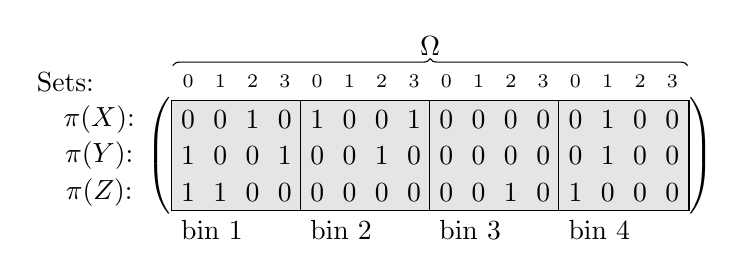
\begin{tikzpicture}[baseline = (M.center),% center with respect to the matrix center
        every left delimiter/.style={xshift=1ex},%tighter delimiter spacing
        every right delimiter/.style={xshift=-1ex}]
\matrix (M) [matrix of math nodes,left delimiter={(},right delimiter={)} 
        ]{ 
0&0&1&0&1&0&0&1&0&0&0&0&0&1&0&0\\
1&0&0&1&0&0&1&0&0&0&0&0&0&1&0&0\\
1&1&0&0&0&0&0&0&0&0&1&0&1&0&0&0\\
};
\node[anchor=south east] (cornernode) at (M-1-1.north west) {Sets: \qquad \qquad}; %Position this more precisely if desired
\foreach[count=\xi] \x in {0,1,2,3,0,1,2,3,0,1,2,3,0,1,2,3}{ %\xi is the counter \x is the value
\node[font=\scriptsize] (M-0-\xi) at (cornernode -| M-1-\xi) {\x}; % Gets the top row 
}
\foreach[count=\xi] \x in {$\pi(X)$:,$\pi(Y)$:,$\pi(Z)$:}{ %\xi is the counter \x is the value
\node (M-\xi-0) at (cornernode |- M-\xi-1) {\x}; %Gets the left most column
}
\node[below left = 0.1pt of M-3-3.south] {bin $1$};
\node[below left = 0.1pt of M-3-7.south] {bin $2$};
\node[below left = 0.1pt of M-3-11.south] {bin $3$};
\node[below left = 0.1pt of M-3-15.south] {bin $4$};

\draw[decoration=brace,decorate] (M-0-1.north west) -- (M-0-16.north east)%
 node[midway,above] {$\Omega$};

\begin{scope}[on background layer]
\draw [fill=black!10] (M-1-1.north west) rectangle (M-3-4.south east);
\draw [fill=black!10] (M-1-5.north west) rectangle (M-3-8.south east);
\draw [fill=black!10] (M-1-9.north west) rectangle (M-3-12.south east);
\draw [fill=black!10] (M-1-13.north west) rectangle (M-3-16.south east);
\end{scope}
\end{tikzpicture}
\end{equation}

The minima-vectors $m(\cdot)$ are
\begin{equation}
\begin{split}
m(\pi(X))=[2,0,*,1],\\
m(\pi(Y))=[0,2,*,1],\\
m(\pi(Z))=[0,*,2,0],\\
\end{split}
\end{equation}
where '$*$' denotes an empty bin.

\section{Conclusions}


\bibliographystyle{unsrt}
\bibliography{Bibliography}

\end{document}